\section{Transfer Learning Across Problem Domains}
\label{sec:deeptune-transfer-learning}

There are inherent differences between the tasks of building heuristics for heterogeneous mapping and thread coarsening, evidenced by the contrasting choices of features and models in \citeauthor{Grewe2013} and \citeauthor{Magni2014}. However, in both cases, the first role of DeepTune is to extract meaningful abstractions and representations of OpenCL code. Prior research in deep learning has shown that models trained on similar inputs for different tasks often share useful commonalities. The idea is that in neural network classification, information learned at the early layers of neural networks (i.e. closer to the input layer) will be useful for multiple tasks. The later the network layers are (i.e. closer to the output layer), the more specialised the layers become~\cite{Zeiler2014}.

Hypothesising that this would be the case for DeepTune would enable the novel transfer of information \emph{across different optimisation domains}. To test this, the language model --- the \texttt{Embedding}, and \texttt{LSTM\_\{1,2\}} layers --- trained for the heterogeneous mapping task was extracted and \emph{transferred} over to the new task of thread coarsening. Since DeepTune keeps the same design for both optimisation problems, this is as simple as copying the learned weights of the three layers. The model is then trained as normal.

As shown in Figures~\ref{fig:pact-speedup-left} and~\ref{fig:pact-speedup-right}, the newly trained model, DeepTune-TL has improved performance for 3 of the 4 platforms: $1.17\times$, $1.23\times$, $1.14\times$, $0.93\times$, providing an average 12\% performance improvement over \citeauthor{Magni2014}. In 81\% of cases, the use of transfer learning matched or improved the optimisation decisions of DeepTune, providing up to a 16\% improvement in per platform performance.

\begin{figure}
  \centering %
  \subfloat[][]{%
    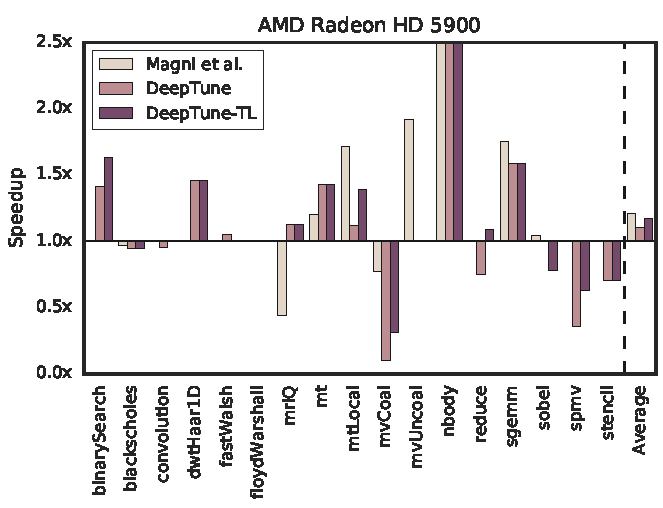
\includegraphics[width=.75\columnwidth]{img/pact-speedup-a}%
    \label{fig:pact-speedup-a}%
  }%
  \\*
  \subfloat[][]{%
    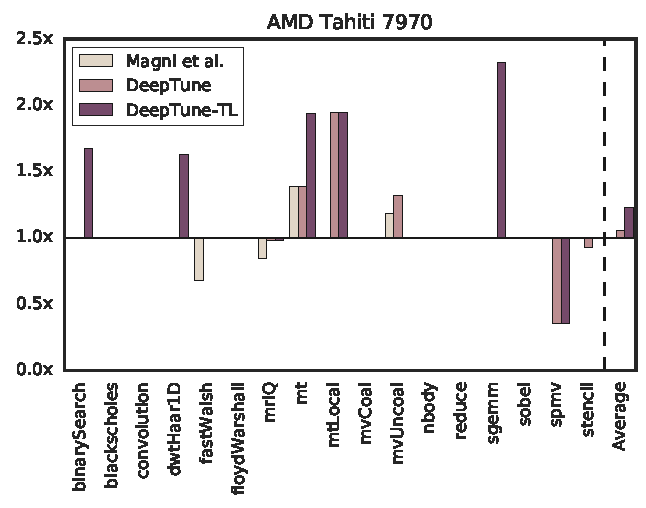
\includegraphics[width=.75\columnwidth]{img/pact-speedup-b}%
    \label{fig:pact-speedup-b}%
  }%
  \caption[Speedups of predicted thread coarsening factors on AMD]{%
    Speedups of predicted coarsening factors on AMD platforms. DeepTune outperforms \citeauthor{Magni2014} on three of the four platforms. Transfer learning improves DeepTune speedups further, by 16\% on average.%
  }%
  \label{fig:pact-speedup-left}
\end{figure}

\begin{figure}
  \centering %
  \subfloat[][]{%
    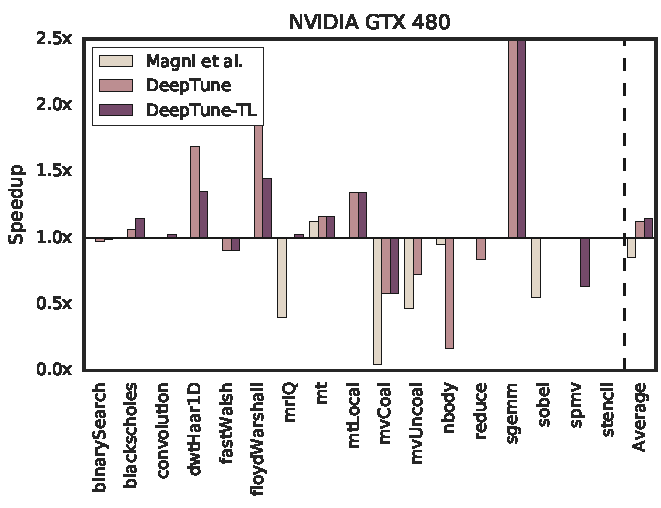
\includegraphics[width=.75\columnwidth]{img/pact-speedup-c}%
    \label{fig:pact-speedup-c}%
  }%
  \\*
  \subfloat[][]{%
    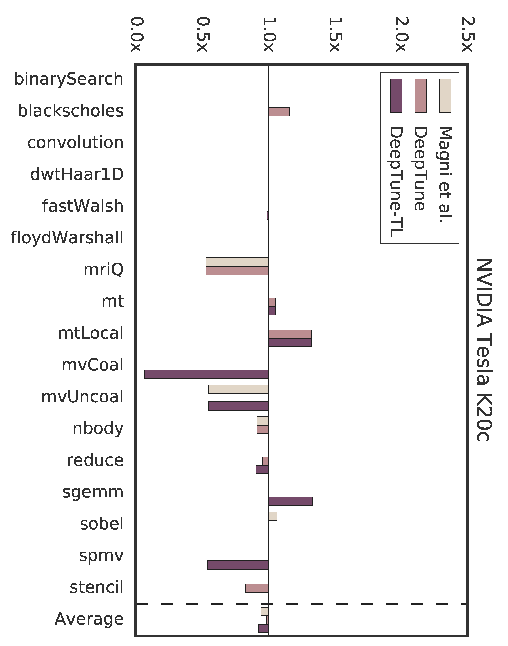
\includegraphics[width=.75\columnwidth]{img/pact-speedup-d}%
    \label{fig:pact-speedup-d}%
  }%
  \caption[Speedups of predicted thread coarsening factors on NVIDIA]{%
    Speedups of predicted coarsening factors on NVIDIA platforms. DeepTune outperforms \citeauthor{Magni2014} on three of the four platforms. Transfer learning improves DeepTune speedups further, by 16\% on average.%
  }%
  \label{fig:pact-speedup-right}
\end{figure}

On the NVIDIA Tesla K20c, the platform for which no predictive model achieves positive average speedups, DeepTune-TL matches or improve performance in the majority of cases, but over-coarsening on three of the programs causes a modest reduction in average performance. For this platform, further performance results are suspected necessary due to its unusual optimisation profile.
